As we saw in Chapter~\ref{chap:mapping}, a central step of model-based software synthesis is a \ac{DSE} step for finding mappings, among others.
We know the mapping space is intractably large and complex and we cannot find the actual optima in the space for any real-life problem sizes.
The best we can hope for are near-optimal mappings in a reasonable amount of time.
Thus, we focus both on the quality of the mappings as well as the time required.
This section will focus on \ac{DSE} for finding near-optimal mappings, as defined in Section~\ref{sec:mapping_problem}. 
We will see many applications of the structures defined and analyzed in Chapter~\ref{chap:mapping_structures}

\subsection{Heuristics and Metaheuristics}
\label{sec:heuristics_vs_metaheuristics}

Generally in \ac{DSE} we distinguish between two approaches for dealing with these kinds of intractable problems, heuristics and meta-heuristics (cf. Section~\ref{sec:mapping_problem}).\index{meta-heuristics}
Recall that mapping heuristics are domain-specific algorithms that exploit the specific domain-knowledge to find a solution based on a pre-defined model of the problem, whereas meta-heuristics rely on an iterative evaluation of the points.
As we outlined above, different heuristics and meta-heuristics come with trade-offs between the exploration time required to find a solution and the quality of said solution.
This is certainly the case for many discrete optimization problems in general, the mapping problem being no exception~\cite{goens_mcsoc16}.
Commonly, meta-heuristics tend to find better results provided enough time, but require accordingly more time to do so.

A particular difficulty of comparing mapping approaches and algorithms are the different models used by different algorithms~\cite{goens_mcsoc16}.
With \mocasin we designed a common framework that allows us to compare between mapping algorithms~\cite{menard_rapido21}.
In particular, in \mocasin we have two heuristics for mapping: the \ac{GBM} heuristic~\cite{castrillon_dac12} and a static mapping variant~\cite{menard_rapido21} of the \ac{CFS} scheduler from Linux.
Additionally, we have implemented genetic algorithms based on and inspired by those found in Sesame~\cite{erbas2006multiobjective,quan2014towards,goens_mcsoc16}, a simulated annealing~\cite{simulated_annealing} mapping algorithm and a tabu search~\cite{tabu_search}.
\index{genetic algorithm}\index{simulated annealing}\index{tabu search}\index{random walk}
We also have a simple random walk algorithm for reference.
A survey of these mapping algorithms, among others can be found in~\cite{singh2013mapping}.
We implemented these algorithms for \mocasin and this thesis to have a basis for comparison from established literature.

We first compare these mapping algorithms to establish a baseline. 
We execute a random walk $500$ random iterations.
For the genetic algorithm we run an evolutionary $\mu + \lambda$ strategy for $20$ generations of population size $10$, crossover rate of $1$ with probability $0.35$ and mutation probability $0.5$, with a tournament selection with tournament size $4$.
For the \ac{GBM} algorithm we set the parameters as \texttt{bx\_m} of $1$, \texttt{bx\_p} of $0.95$, \texttt{by\_m} of $0.5$,\texttt{by\_p} of $0.75$, 
The simulated annealing heuristic we execute with an initial temperature of $1$ and a final temperature of $0.1$, with a temperature proportionality constant of $0.5$  and a random movement starting radius of $5$.
Finally, for the tabu search mapper we set a maximum of $30$ iterations, each of size $5$ and with a move set size of $10$ and tabu tenure of $5$, and a random candidate move update radius of $2$.
These parameters were chosen such that the mappers seemed to yield good result, yet not systematically (e.g. using something like Bayesian optimization or general (hyper-)parameter optimization approaches).
A deliberate choice in the parameters however is that the exploration times should be comparable between the meta-heuristics, i.e. such that the iterative mappers evaluate a similar amount of mappings.

\begin{figure}[h]
	\centering
   \resizebox{0.95\textwidth}{!}{\input{generated/heuristics_vs_metaheuristics.tex}}
	\caption{Comparison of multiple mapping heuristics and metaheuristics on the \ac{E3S} benchmarks.}
	\label{fig:heuristics_vs_metaheuristics}
\end{figure}

Figure~\ref{fig:heuristics_vs_metaheuristics} shows a comparison of the different heuristics and metaheuristics on the \ac{E3S} benchmarks.
Each of the metaheuristics that require random data we execute $10$ times and show the variation as calculated by the unbiased estimator of the standard deviation of the multiple sampled times.
The execution times vary obviously depending on the different benchmark applications and on the platforms they run on.
The absolute values of these times, however, are not interesting for comparing the mapping algorithms.
We thus norm the values of the execution times, taking the results of the genetic algorithms as baseline.
We then aggregate all values with the geometric mean.
The error bars in the plot are calculated by taking the average value $\pm$ the estimated standard deviation and norming each of the two extremes, the results of which are the extremes shown in the plot.

We first examine the results for the Odroid XU4 architecture.
The two heuristics find considerably lower results in average, but they do so in considerably less time.
More concretely, they yield about an order of magnitude worse results in about an order of magnitude less time.
The results of the random walk heuristic are significantly worse than those of the more structured metaheuristics, even though it takes a comparable amount of time.
This is due to a deliberate choice, since as explained above, the number of random mappings was chosen specifically to be comparable to the number the number of mappings evaluated by the other meta-heuristics.
Since $500$ mappings is not a small amount, it is not terribly surprising that the random mapper beats the two heuristics.
Finally, the best mappings are found by the simulated annealing meta-heuristic, albeit only by $3\%$ compared to the genetic algorithm.

When we turn our attention to the significantly larger and more complex MPPA3 Coolidge architecture, we see that the picture changes drastically.
The marked difference between heuristics and meta-heuristics disappears in this case.
The \ac{GBM} heuristic is on par with the random walk results in average, while taking substantially less time.
This is simply explained by the significantly larger design space of mapping to the MPPA3 Coolidge.
In this case, the genetic algorithm significantly outperforms both other meta-heuristics, by a factor of $4-5$, while taking less time.
The most striking result here, however, is the extremely good performance of the static CFS heuristic.
This good performance is misleading at first, a perhaps more honest assessment of the results is that \emph{all other (meta-) heuristics perform poorly}.
We can interpret this as a consequence of the growing design space and its complexity, which affects the metaheuristics, while the static CFS mapper can still leverage domain-specific knowledge to find fairly good mappings.

%TODO: add and test genetic with CFS initials.

\subsection{Leveraging Symmetries}

As motivated when discussing them in Section~\ref{sec:symmetries}, symmetries can be used to improve \ac{DSE} in the mapping problem.
There are two distinct applications of symmetries in \ac{DSE}.
The first application is for speeding up meta-heuristics (without modifying them), as shown in~\cite{goens_taco17}, by leveraging the equivalence of symmetric mappings in a symmetry-aware cache.
The second application is by pruning the design space as seen by the meta-heuristic~\cite{goens_mcsoc18,goens_tcad21}, effectively changing the meta-heuristic.

We will first discuss the idea of a symmetry-aware cache.\index{symmetry-aware cache}
As discussed before, meta-heuristics work through an iterative principle, where they evaluate mappings and drive the search based on the results of the evaluation.
While the evaluation is fast and light-weight by design (cf. sections~\ref{sec:sec:simulating_mappings} or~\ref{sec:architecture_models}), it still usually dominates the execution time of the exploration (cf. Figure~\ref{fig:heuristics_vs_metaheuristics}).
A defining property of the symmetries is how simulation results are invariants of the equivalence classes of orbits (cf. Section~\ref{sec:symmetries}).
This means that if we know the results of a simulation for a mapping, we know the results for all mappings in its equivalence class.
We can leverage this by designing a symmetry-aware mapping cache, which stores simulations results by equivalence class instead of by mapping~\cite{goens_taco17}.
This yields a trade-off, where computations about the symmetry have to be executed every time a mapping is going to be looked-up in the cache or evaluated.

We implemented a symmetry-aware cache in \mocasin which uses \mpsym and its Python interface.
We used this to evaluate the method of symmetry-aware caching on the \ac{E3S} benchmarks by accelerating the various meta-heuristics discussed in Section~\ref{sec:heuristics_vs_metaheuristics}.
We can also evaluate the domain-specific methods of mpsym~\cite{goens_tcad21} by applying this method to multiple architecture topologies.
In addition to the Odroid XU4 and MPPA3 Coolidge, which we used consistently throughout this thesis, we also test the methods on the exploration of two additional architectures: \ac{HAEC} and a simple generic cluster.
The \ac{HAEC} architecture (cf. Figure~\ref{fig:HAEC}) is a \ac{PCB} design with low-latency optical interconnects on layers with a $4 \times 4$ regular-mesh structure.
Four such layers are then connected, using low-latency wireless interconnects to communicate between adjacent layers.
While in the \ac{HAEC} design each node of the layer is an \ac{MPSoC}, we model the topology by placing cores in those nodes and considering the board as a single \ac{MPSoC}.
This serves to evaluate our methods on this topology.
The generic cluster architecture we evaluate is the simplest non-trivial clustered architecture topology.
It consists of two identical clusters, each of which with two identical cores.
Each cluster shares a cache, and the two clusters can communicate over main memory.

To manage the sheer amount of experiments ($\gg 10^5$) for this evaluation and the upcoming ones in this chapter, we modified slightly modified the parameters of the meta-heuristics, reducing the overall execution time.
We reduced the number of generations of the genetic algorithm to $10$, the number of iterations of the random walk to $300$, reduced the initial temperature of the simulated annealing heuristic to $0.1$ and the maximum number of iterations of the tabu search algorithm to $5$, with an increased radius of $2.5$.

\begin{figure}[h]
	\centering
   \resizebox{0.95\textwidth}{!}{\input{generated/symmetries_cache.tex}}
	\caption{The effect of a symmetry-aware cache on multiple architecture topologies as evaluated on the \ac{E3S} benchmarks.}
	\label{fig:symmetry_cache}
\end{figure}


Figure~\ref{fig:symmetry_cache} shows the results of evaluating a symmetry-aware cache on the different meta-heuristics on different architecture topologies.
It reports the execution time of the full exploration, separating the overhead from symmetry calculations from the rest of the exploration time for the symmetry-aware cache.
These relative times are normed such that the regular exploration has a time of $1$. Both variants were executed $10$ times with identical seeds, for each benchmark. 
Thus, they executed the exact same exploration, evaluating the exact same mappings and returning the same result.

Unsurpisingly, the symmetry-aware cache does not offset the overhead of symmetry calculations for the random walk meta-heuristic.
Since the mapping space is extremely large, the probability of finding two equivalent mappings at random is quite small. 
Thus, both a symmetry-aware cache and a regular cache are not very useful for an unstructured random walk.
The other meta-heuristics are much more structured, and clearly do benefit from the speedup.
For the Odroid XU4, the symmetry-aware cache consistently yields a large speedup of the exploration time, around $1.4-1.7 \times$.
For the simple cluster and the \ac{HAEC} architectures, the results are similar.
The best results are achieved for the MPPA3 Coolidge topology, which despite its complexity has a very well-defined structure we can exploit with our wreath-product construction (cf. Section~\ref{sec:symmetries}).
For the simulated annealing meta-heuristic, our symmetry-aware cache sped up the simulation in \textbf{average} by $14.5 \times$!

We see that our \mpsym-powered symmetry-aware cache is very useful for speeding up \ac{DSE}.
It can still be improved, however.
In~\cite{goens_taco17} we also included application symmetries in the cache, which actually made a significant difference, as we were not using the more optimized algorithms from \mpsym.
Application symmetries have a much potential, which is also intuitive if we consider the cardinality of the mapping space $|V_A|^{|V_K|}$ grows exponentially with the number of processes.
However, as explained in Section~\ref{sec:app_arch_symmetries}, we have no systematic method of reliably detecting these application symmetries yet, which is why we do not include them in \mocasin.
The other improvement comes from partial permutations. While we described them in Section~\ref{sec:partial_symmetries} and have a partial implementation in \mpsym, we still need efficient algorithms on partial permutations for exploiting the partial symmetries of the mapping space.
This is evident in the comparison between the results of the MPPA3 Coolidge and \ac{HAEC} topologies in Figure\ref{fig:symmetry_cache}.
The \ac{HAEC} topology has partial symmetries in each of the meshes (cf. Section~\ref{sec:partial_symmetries}), and it also has partial symmetries in the symmetry group of the clusters (the larger group from the wreath product).
Since the first and last layers cannot communicate with each other directly (the topology is not toric), the symmetries of the clusters are all only partial.

We can also leverage symmetries in \ac{DSE} by changing the underlying space as seen by the meta-heuristic.
We also implemented this in \mocasin by using the \texttt{SymmetryRepresentation} as described in Section~\ref{sec:representations}.
In this way, the meta-heuristics see the factor space and are effectively changed in their operations.

\begin{figure}[h]
	\centering
   \resizebox{0.95\textwidth}{!}{\input{generated/symmetries_changed_operations.tex}}
	\caption{The effect of a symmetry-aware cache on multiple architecture topologies as evaluated on the \ac{E3S} benchmarks.}
	\label{fig:symmetry_changed_operations}
\end{figure}

We tested this with the same setup as before, the results of which can be seen in Figure~\ref{fig:symmetries_changed_operations}.
It shows both, the relative results of the mapper (in terms of the runtime of the best mapping) and the relative exploration times.
The times shown are relative to the random walk meta-heuristic in the regular implementation, i.e. without symmetries.
It is not surprising that most times for the best mapping results are thus $<1$, as the random walk meta-heuristic is not as good as the other meta-heuristics.
The more interesting comparison, however, is between both variants of each mapping algorithm.
For the simpler platforms, Odroid-XU4 and the simple cluster  the symmetry-enabled variant speeds up the execution in a fashion similar to the symmetry-enabled cache, while yielding similar results.
For the more complex platforms, \ac{HAEC} and the Kalray MPPA3 Coolidge, the results vary between both.
The results of the mapping algorithm are considerably better on the MPPA3 Coolidge, while being very similar for both representations in the \ac{HAEC} platform.
The exploration time was also improved consistently for both platforms.
The difference between the results for the \ac{HAEC} and MPPA3 Coolidge platform can again be explained by the missing partial symmetry support in the implementation.

The performance improvement for the MPPA3 Coolidge, however, is very impressive.
For the simulated annealing meta-heuristic, the mappings found for the \ac{E3S} benchmarks were an \emph{average} of $32.4 \times$ better with the symmetries than without them.
This impressive result is, as we have seen in Figure~\ref{fig:heuristics_vs_metaheuristics}, rather a testament of how badly the meta-heuristic performs without the symmetries in this complex architecture.
To understand the mapping results for the MPPA3 Coolidge, Figure~\ref{fig:symmetry_coolidge_changed_operations} shows the results for this platform in more detail.
Instead of separating the benchmark by domain (cf. Table~\ref{tab:e3s}), we separate them by the number of tasks in the task graph.
The number of tasks is a metric that better describes the complexity of the mapping space. 
In this case the values are normed to the regular variant of the algorithm for each algorithm, instead of norming all values relative to a single algorithm.

\begin{figure}[h]
	\centering
   \resizebox{0.95\textwidth}{!}{\input{generated/symmetries_coolidge_changed_operations.tex}}
	\caption{The effect of a symmetry-aware cache on multiple architecture topologies as evaluated on the \ac{E3S} benchmarks.}
	\label{fig:symmetry_coolidge_changed_operations}
\end{figure}

It is obvious that the symmetries are not advantageous for a random mapping, as explained before due to the sheer size of the mapping space.
This is clearly visible in Figure~\ref{fig:symmetry_coolidge_changed_operations}.
For the algorithms based on tabu search and simulated annealing, the advantage comes predominantly for smaller task graphs (with $2-5$ tasks).
For larger tasks probably the symmetries are not as effective anymore and both variants perform poorly. 
The genetic algorithm seems to continue to profit from the symmetries for larger task graphs, but it is conceivable that this advantage would still not hold for task graphs larger than those found in the \ac{E3S} benchmarks.

\subsection{Leveraging Metric Spaces}

The same way we used the \texttt{Symmetry} representation to improve \ac{DSE}, we can use the \ac{MetricSpaceEmbedding} representation and see if this improves the performance of mapping algorithms.
The two meta-heuristics that are primarily based on an underlying metric space structure of the search space are tabu search and simulated annealing.
We compare the results of these two meta-heuristics on both the \ac{E3S} and \ac{CPN}-based benchmarks.
For each meta-heuristic, each representation and each benchmark application, we measure the results of $10$ runs with different random seeds.

\begin{figure}[h]
	\centering
   \resizebox{0.95\textwidth}{!}{\input{generated/geometric_heuristics_coolidge.tex}}
	\caption{The effect of embedding-based representations in metaheuristics that leverage the geometry on the MPPA3 Coolidge platform.}
	\label{fig:coolidge_geometric}
\end{figure}

Figure~\ref{fig:coolidge_geometric} shows the results of this experiments for the MPPA3 Coolidge platform, where we have seen before that the metric space structure of our embedding-based representations is better than the canonical metric in the \texttt{SimpleVector} representation.
We see that the results of the exploration are significantly better for both meta-heuristics with the representations based on this better distance metric.
This modest improvement does come at a cost in exploration time, which is clearly attributable to the increased dimension of the embedding spaces in these representations.
We have also seen in the previous results that these meta-heuristics perform poorly for the MPPA3 Coolidge with its complex topology and large design space.

The results still provide some insight into the nature of the design space and the usefulness of the embedding-based representations.
We can concretely make two observations from these results and combine them to produce a new meta-heuristic.
The first one is the knowledge that geometry-based heuristics indeed benefit from a better metric, independent of if the resulting heuristics are overall good.
The second observation is more subtle, it's about the general structure of the design space. 
The design spaces of mappings seem to consist of multiple islands of performance with similar properties, separated by poorly-performing mappings.
This is apparent already in the extremely simple two-task example in Figure~\ref{fig:mapping_space_full}.
The visualization with the methods from~\cite{visualloss} in Figure~\ref{fig:mapping_space_visualization} or in Figure~\ref{fig:visualization_design_centering_spaces} makes this even more apparent.

The idea behind the representations is leveraging the underlying structure of the design space.
As such, these ``performance islands'' seem to be reduced by both representation methods discussed here, as is also suggested by Figure~\ref{fig:mapping_space_full}.\index{performance islands}
We also applied the methods from~\cite{visualloss} to the same design space of the \texttt{audio filter} benchmark on the MPPA3 Coolidge with the \texttt{SymmetryEmbedding} representation.
Figure~\ref{fig:visualization_simpvec_symemb} shows the results of this visualization alongside the same mapping space visualization for the \texttt{SimpleVector} representation, reinforcing the intuition of these ``performance islands''.

\begin{figure*}[t]
  \centering
	\begin{subfigure}[b]{0.43\textwidth}
    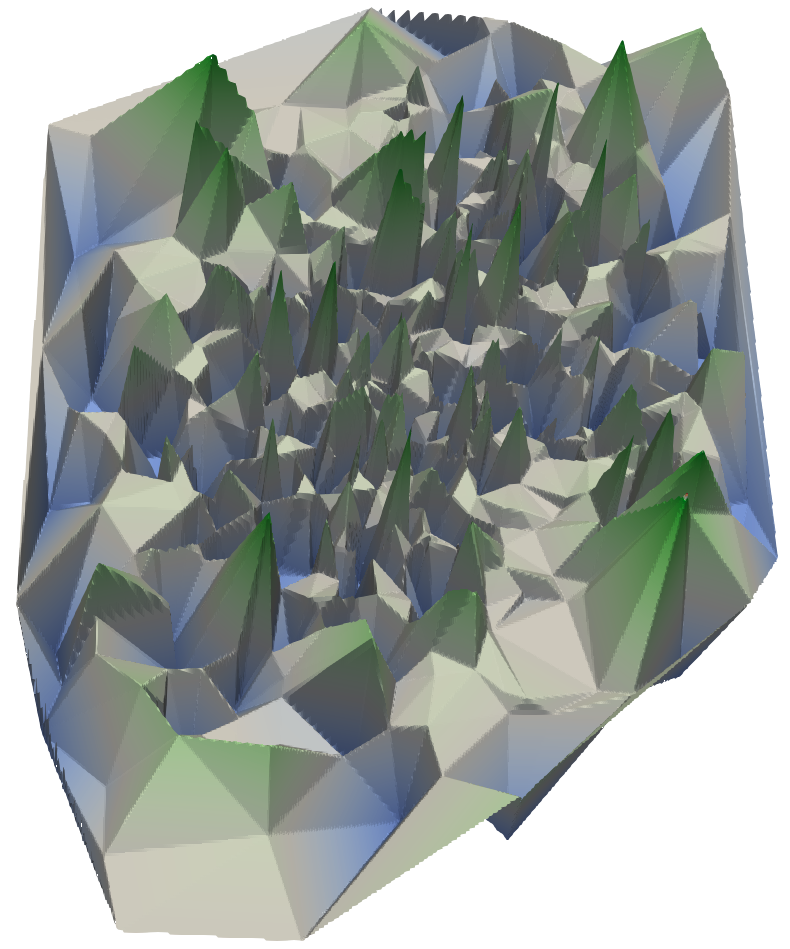
\includegraphics[width=\textwidth]{figures/coolidge-af-space-sim-vec.png}
		\caption{SimpleVector}
	\end{subfigure}
	~
	\begin{subfigure}[b]{0.43\textwidth}
    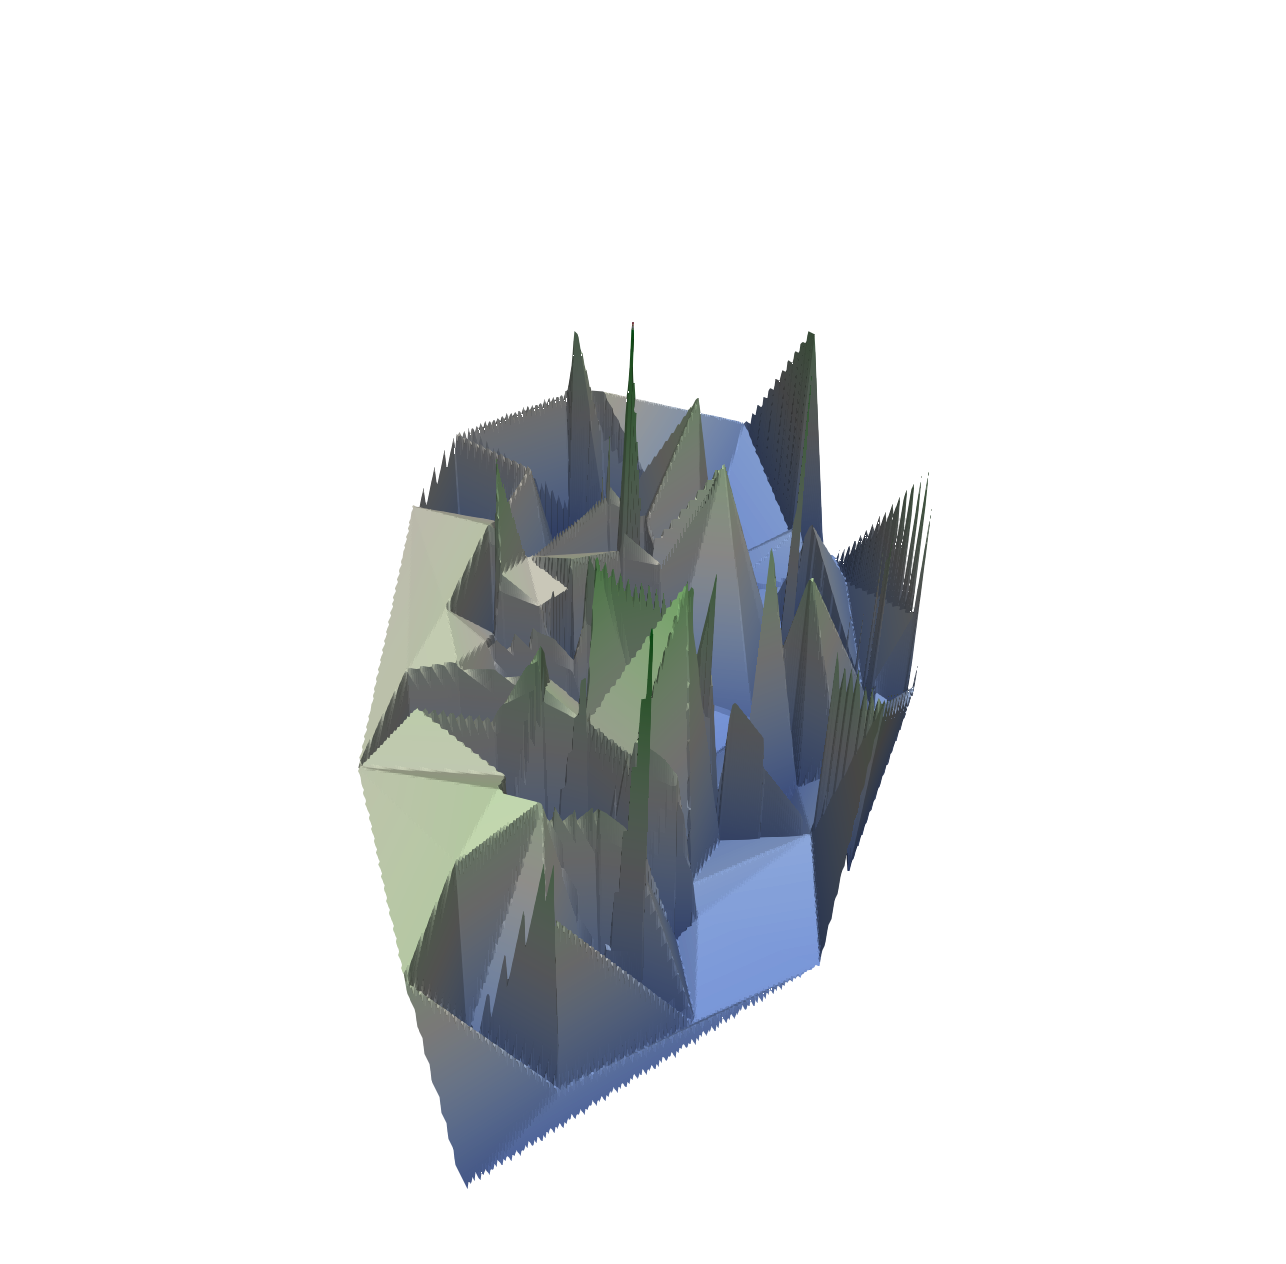
\includegraphics[width=\textwidth]{figures/coolidge-af-space-emb-sym.png}
		\caption{SymmetryEmbedding}
	\end{subfigure}

	\caption{Visualization of the same design space of the audio filter benchmark on the MPPA3 Coolidge platform in two different representations.}%
	\label{fig:visualization_simpvec_symemb}
\end{figure*}


The best indicator of this, however, are the vertical lines in the relative distances from the metric spaces (cf. Figure~\ref{fig:metric_comparison_exynos} and Figure~\ref{fig:metric_comparison_coolidge}).
Since the abscissa in these two plots represents the (relative) mapping distance in the corresponding metric, vertical lines indicate equidistant points. 
The fact that there are points with the full range of relative execution times in these equidistant ranges is consistent with such ``performance islands''.
If the mapping space landscape was more regular, the plots would more closely resemble those where we only considered the maxima (cf. Figure~\ref{fig:metric_comparison_max_exynos} and Figure~\ref{fig:metric_comparison_max_coolidge} respectively).

We can use this observation to derive a new meta-heuristic for exploring the mapping space.
Our ``performance islands'' hypothesis implies the mapping space is full of local minima.
Guiding a local search towards an optimum should thus not be as conducive to good results.
Instead, we can use a simple and fast meta-heuristic to find a local minimum quickly and apply it to multiple points spread around the design space's geometry. 
As meta-heuristic for finding local minima we use the well-known gradient descent optimization algorithm with the momentum method~\cite{rumelhart1986learning}.
For the step-size we use the Barzilai-Borwein \cite{barzilai1988two} method.
In its regular form this heuristic will quickly get stuck in a local minimum and produce poor mapping results, as confirmed by experiments (which we omit here).
However, we can add a simple additional meta-heuristic to leverage the ``performance islands'' hypothesis.
We start the heuristic at multiple random points, uniformly distributed in the design space, as defined the distance metric.
In these spread-out locations we execute (parallel) gradient descent optimizations which we cancel as soon as they reach a local minimum, which empirically happens after a handful of iterations.
The meta-heuristic returns the fastest mapping found in any of the different starting locations.
We configure the meta-heuristic to run on $5$ different locations with a maximum of $20$ iterations each, even though this maximum is almost never reached in practice in the experiments.

%\subsection{All Representations}
\begin{figure}[h]
	\centering
   \resizebox{0.95\textwidth}{!}{\input{generated/multiple_representations_exynos.tex}}
	\caption{Comparison of the effects of multiple representations on the Odroid XU4 platform.}
	\label{fig:multiple_representations_exynos}
\end{figure}

Figure~\ref{fig:multiple_representations_exynos} shows a comprehensive comparison on the Odroid XU4 platform for both benchmarks of all meta-heuristics, including our new islands-based gradient descent method. 
The results reflect our previous results (cf. figures~\ref{fig:symmetry_changed_operations} and~\ref{fig:heuristics_vs_metaheuristics}).
We see that the embedding-based representations yield worse results for tabu search and simulated annealing, and require more time in almost all cases.
These representations are not very useful for this platform, which is consistent with the previous results.
The more interesting results are for those for the considerably more complex topology of the MPPA3 Coolidge.

\begin{figure}[h]
	\centering
   \resizebox{0.95\textwidth}{!}{\input{generated/multiple_representations_coolidge.tex}}
	\caption{Comparison of the effects of multiple representations on the MPPA3 Coolidge platform.}
	\label{fig:multiple_representations_coolidge}
\end{figure}

Figure\ref{fig:multiple_representations_coolidge} shows the same comprehensive comparison of all meta-heuristics and all representations on all benchmarks, this time for the MPPA3 Coolidge platform. 
Besides from the results already seen and discussed before in figures~\ref{fig:symmetry_changed_operations},~\ref{fig:heuristics_vs_metaheuristics} and \ref{fig:coolidge_geometric}, the most notable results are the results for our new island-based gradient descent meta-heuristic.
Despite its simplicity, this meta-heuristic significantly outperforms all the other more sophisticated meta-heuristics.
The two embedding-based representations yield worse results, which is consistent with our ``performance islands'' hypothesis.
In a more structured design space it is more difficult to find the better performance islands than in a less structured one which features good mappings in more islands.
The \texttt{Symmetries} representation yields the best results, which is also consistent with this, as it only reduces the size of the design space without fundamentally changing its topology.
In a smaller space it is more likely to find an island with a higher local minimum.

\begin{figure}[h]
	\centering
   \resizebox{0.7\textwidth}{!}{\inputTikz{2d_mapping_heatmap_orig}}
	\caption{The actual mapping space of  GSM two-task application from \ac{E3S} on the Odroid XU4 that inspired Figure~\ref{fig:mapping_space_example}.}
	\label{fig:gsm_actual_mapping_space}
\end{figure}


Recall the intuition of Figure~\ref{fig:mapping_space} of all representations for the simple two-task example.
We can see how the \texttt{Symmetries} representation has two islands, with fast mappings, whereas the \ac{SymmetryEmbedding} representation only has one.
For such a simple example the symmetries capture all different execution times.
In the original task graph, a \ac{GSM} application from the \ac{E3S} benchmarks, the differences in execution times were much lower. 
Figure~\ref{fig:gsm_actual_mapping_space} shows the actual mapping space. Since the differences in execution times are barely visible from the color coding, the times (in ms) are also explicitly written in the figure to show the differences.
This shows one of the limitations of the symmetries and a possible explanation for the ``performance islands'' hypothesis: many mappings are not equivalent, but very similar.
In future work we could capture these similarities in mappings in a more formal fashion.
This should allow us to better explore the design space.